\section{FreMEn - Predicting future occupancy}
\label{sec:fremen}
The  Frequency Map Enhancement (FreMEn) method models the dynamics of each cell by its primary frequency components. It has successfully been applied to improve mobile robots ability to perform feature-based localization \cite{online_fremen} and topological navigation \cite{fentanes2015}. Here Krajník et al. argues for approximating the appearance and disappearance of obstacles with multiple periodic sinus signals, since people often moves them as part of daily routines. As discussed in section \ref{sec:characteristics_in_industrial_environments} this might also be the case in the industrial environments in focus here. Resent work in \cite{life_long_exploration}, shows how the often violated assumption in FFT about a fixed sampling rate is met by incrementally adding sparse and irregular observations. Where the approach usually uses the number of frequency components(m) that minimizes the difference between predicted states and measurements, it is chosen to use the typical order m=2 \cite{life_long_exploration} for all cells. This will probably decrease the prediction performance, but enables online updates without having to store observations for evaluation.

The online variant of the approach updates the parameters shown in equation \ref{eq:fremen_time} for each new measurement $s(t)$. 
The average occupancy probability $\alpha_0$ models the $0Hz$ signal and is updated with a new measurement online. 
The number of measurements n is incremented. There is one of the complex numbers $\gamma_k$ and $\beta_k$ for each $\omega_k=1/T_k$ . 
$T$ is calculated with equation \ref{eq:fremen_update} for each frequency, where N is the 20 used frequency components and epsilon is the smallest period time, which is one minute here. 
The values of consecutive $T_k$ is close for large values of $k$, which is advantageous if most of the obstacles moves with a period close to $\epsilon$.

\begin{equation}
    T_k = \frac{N \epsilon}{k+1}
    \label{eq:fremen_time}
\end{equation}

The real and imaginary part of $\gamma_k$ and $\beta_k$ are updated as the running average. $\gamma_k$ is the part of the signal with the frequency $2 \pi \omega_k$ and $\beta_k$ is the part of this signal which are modeled by the $0Hz$ component of the signal.

\begin{eqnarray}
&\alpha_0 = \frac{1}{n+1}(n \alpha_0 + s(t)) \nonumber \\ 
&\gamma_k = \frac{1}{n+1}(n \gamma_k + s(t) e^{-j \omega_k t}) \forall \omega_k \in \Omega  \\
&\beta = \frac{1}{n+1}(n \beta_k + \alpha_0 e^{-j \omega_k t}) \forall \omega_k \in \Omega \nonumber \\
&n = n + 1 \nonumber
\label{eq:fremen_update}
\end{eqnarray}

When predicting the state of a cell at time $t$ the signal components are calculated with equation \ref{eq:fremen_freq_component}.

\begin{equation}
    \alpha_k = \gamma_k - \beta_k \forall \omega_k \in \Omega
    \label{eq:fremen_freq_component}
\end{equation}

Then $ \Omega $ is ordered based $ | \alpha_k | $ to enable calculation of equation \ref{eq:fremen_predict} using only the $m$ most prominent frequency components. As previously described, we use two frequency components ($ m=2 $) for each cell.

\begin{equation}
p(t) = \zeta \left( \alpha_0 \sum_{k=1}^{m} |\alpha_k| cos(\omega_k t + arg(\alpha_k))  \right)
\label{eq:fremen_predict}
\end{equation}

The function $\zeta$ clamps the expected probability to a value between zero and one. The $arg$-function returns the angle of the complex number with respect to the x-axis.
The occupancy state at time $t$ is predicted as occupied if $p(t)$ is above $0.5$ and as free otherwise.

\begin{figure}[htbp]
\centering
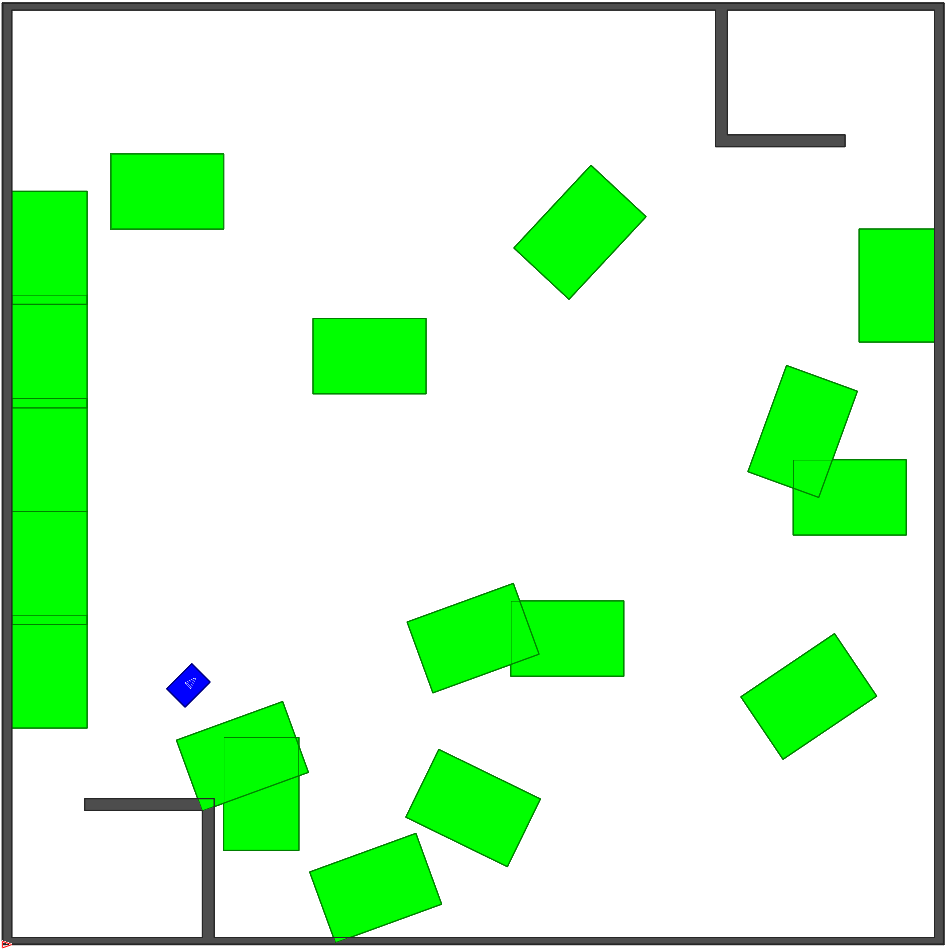
\includegraphics[width=0.4\linewidth]{chapters/mapping_of_dynamic_areas/figures/simulated_environment}
\caption{Screen shot of Stage simulator showing a MIR 100 robot navigating around obstacles which appears and disappears at fixed intervals.}
\label{fig:simulated_environment}
\end{figure}

The methods ability to predict future occupancy states are evaluated in a Stage simulation where many boxes moves in and out at various and fixed, intervals. 
The robot continuously navigates from the lower left corner that are partly surrounded by walls to the top right corner, while the red and green boxes moves around.
The measurements from the simulated LIDAR are incorporated in a temporary local map using the reduced ideal inverse sensor model update method described in section \ref{sec:reduced_ideal_sensor_model}. 
The update values for the sensor model is reduced to incorporate uncertainties in localization.
For every fifth second a global map of FreMEn cells are updated with \ref{eq:fremen_update} where $s(t)$ is the probability for occupancy in the local map. 
The local map is then cleared and the process continues.

\begin{figure}[htbp]
    \centering
    \begin{subfigure}[t]{0.49\textwidth}
        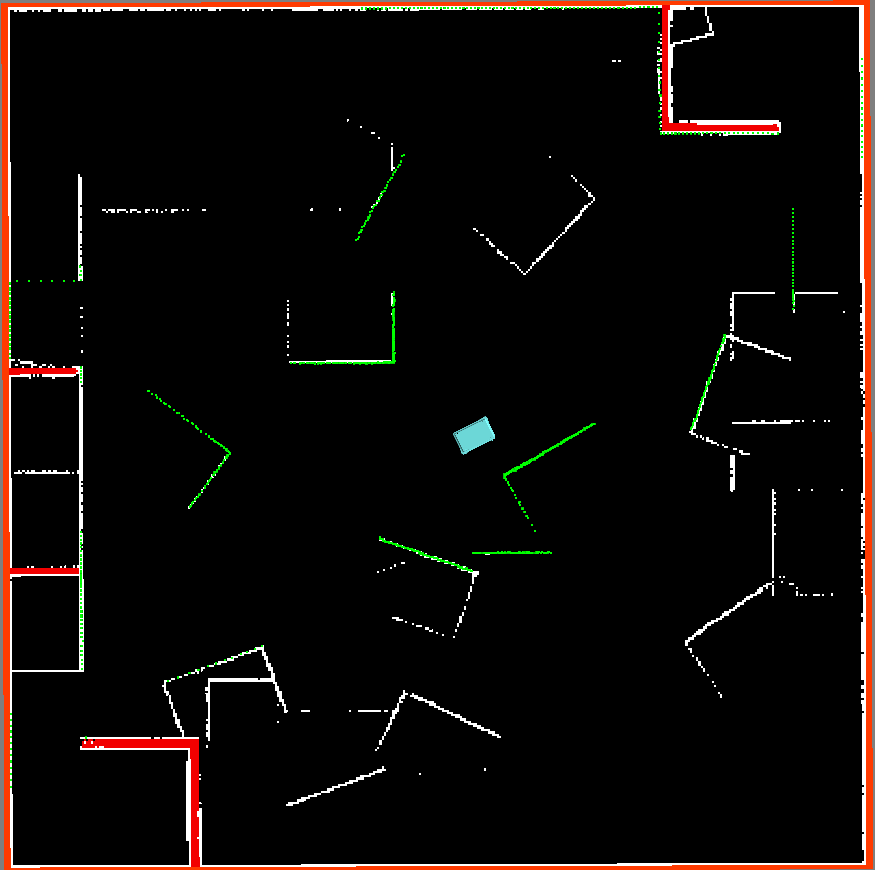
\includegraphics[width=1.0\textwidth]{chapters/mapping_of_dynamic_areas/figures/fremen_ideal_simulation}	
        \caption{Predicted map without noise.}
        \label{fig:fremen_ideal_sim}
    \end{subfigure}
    \begin{subfigure}[t]{0.49\textwidth}
        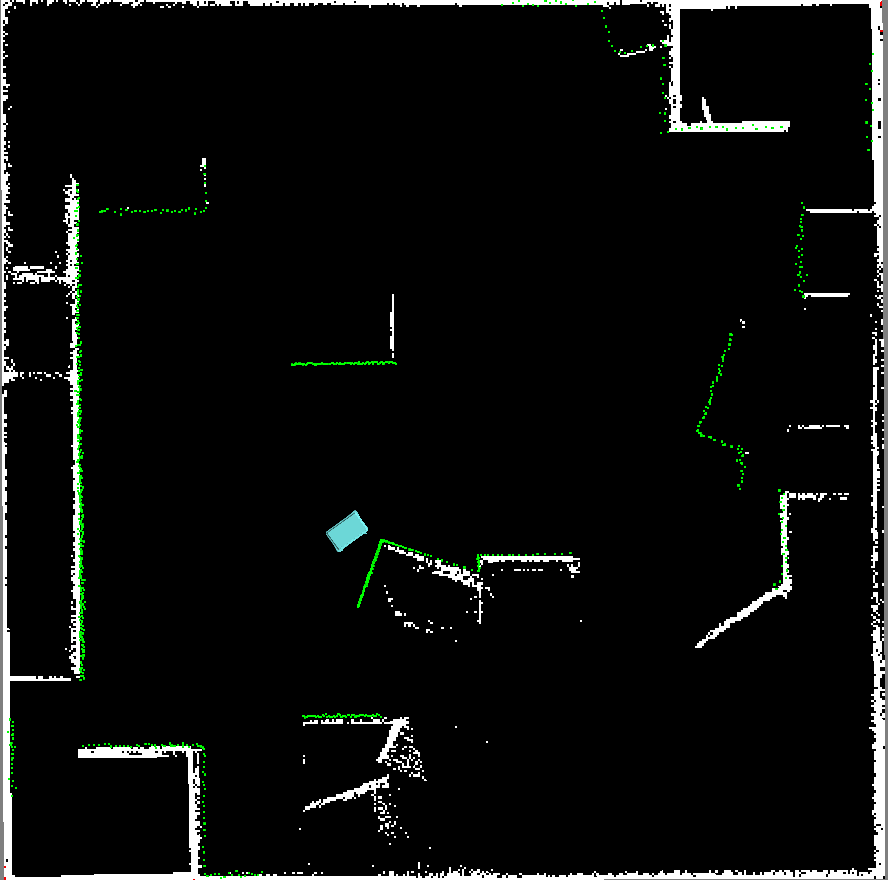
\includegraphics[width=1.0\textwidth]{chapters/mapping_of_dynamic_areas/figures/fremen_with_decay_last}
        \caption{Predicted map with realistic sensor and localization noise.}
        \label{fig:fremen_sim_with_noise}
    \end{subfigure}
    \caption{Robot navigating in the map predicted with FreMEn where the the green dots marks ends of LIDAR readings.}
\end{figure}

To evaluate the predictive strength of FreMEn it is used to predict the appearance of obstacles each time a new measurement is added from the local map. 
Figure \ref{fig:fremen_ideal_sim} shows how FreMEn correctly predicts the appearance of many of the obstacles when the robots exact position is used to incorporate exact LIDAR measurements. 
Figure \ref{fig:fremen_avg_miss_with_noise} shows a more realistic simulation with Gaussian noise on LIDAR measurements with a standard deviation of one centimeter and localization using AMCL with a static map representation.
Here some of the obstacles are predicted to have moved while they in fact are still present, as shown in the middle to the right in figure \ref{fig:fremen_avg_miss_with_noise}.

FreMEn's lack of ability to predict future measured obstacles is also apparent in the average correctly predicted observations of obstacles. 
This is shown in figure \ref{fig:fremen_avg_correct_predictions} where the good prediction percent on $74.0\%$ drops to $46.9\%$ with the addition of noise.
From the experiment without noise it is concluded that the learned periodic appearance of obstacles in a grid with FreMEn is useful for predictions.
In the presence of noise the signals within the cells becomes more complicated, and the measurements used for comparison is not always correct.
This, combined with the fact that obstacles placed by humans probably will not move in and out of grid cells so consistently as in this simulation, leads us to believe that the implemented method is not useful for online update of the occupancy grid map used by AMCL.
It might however be possible to alter the method, or combine it with others, to take advantage of the methods ability to predict presence of obstacles many hours after the last observation.
The predicted maps can improve the validness of global paths planned by the robot, but with the rather poor prediction percentage many paths have to be re-planned during navigation. 

\begin{figure}[htbp]
    \centering
    \begin{subfigure}[t]{0.49\textwidth}
        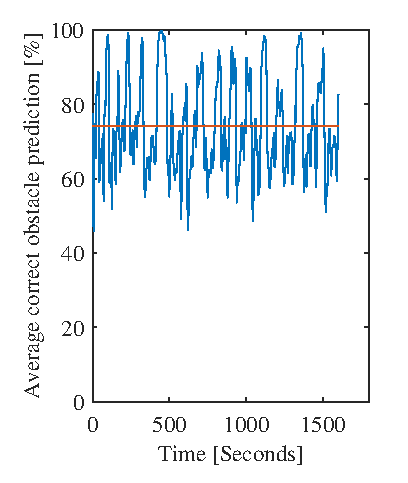
\includegraphics[width=1.0\textwidth]{chapters/mapping_of_dynamic_areas/figures/fremen_avg_miss_no_noise}	
        \caption{Prediction score without noise.}
        \label{fig:fremen_avg_miss_no_noise}
    \end{subfigure}
    \begin{subfigure}[t]{0.49\textwidth}
        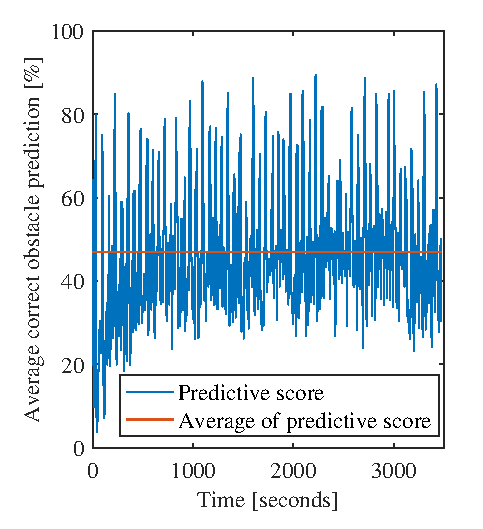
\includegraphics[width=1.0\textwidth]{chapters/mapping_of_dynamic_areas/figures/fremen_avg_miss_with_noise}
        \caption{Prediction score with noise.}
        \label{fig:fremen_avg_miss_with_noise}
    \end{subfigure}
    \caption{Prediction scores for FreMEn defined as the average number of matches between measured and predicted obstacles.}
    \label{fig:fremen_avg_correct_predictions}
\end{figure}
